\section{Overall Description}

%  in automatico Section [number]
\subsection{Product
perspective}
Here we discuss in details all the shared phenomena outlined in Section 1.2 and we also provide a domain model through class and state diagrams.
\\\newline
    \noindent\textbf{Shared Phenomena, controlled by the world and observed by the machine. }
\begin{itemize}
    \item Register/login: a Guest can register to the application through an intuitive form; Authorities login in made using already existing credentials, they don't need a registration;
    Users can login to the application through an intuitive form;
    \item Report of a traffic violation: the User is able to report traffic violations at any time, he/she can open the application and then send the report including the picture, the type of violation and the name of the street where the violation occurred.
    \item The Municipality offers up-to-date information about urban mobility; in this way the System can cross this information with its own ones. 
\end{itemize}

\vspace{10px}

    \noindent\textbf{Shared Phenomena, controlled by the machine and observed by the world.}
      \begin{itemize}
      % controllare se forwarding va bene
          \item Authorities can access reports: the reports sent by Users are collected by the System; the Authorities accessing the application can view them.
          \item Visualization of own reports: the System allows Users to view their reports.
          \item Visualization safe/unsafe areas: the System through the service offered by the municipality is able to get a list of areas in which accidents took place, thus the System can show unsafe and safe areas to the User.
          \item Suggest possible interventions: the System,  by using a list of known and effective solutions for some common violations, is able to suggest possible interventions in order to reduce the number of violations and make unsafe areas more safe.
          \item Notify about corrupted pictures: if the User modifies a photo in order to send malicious reports, the System marks the report as corrupted and the User as a potential malicious one.
          \item Generate Statistics: the System is able to generate chart that illustrate statistics, like the most egregious offenders and the effectiveness of the application itself.
          \item System manages multiple Reports of the same traffic violation: if the System recognizes that a report there is going to be made, refers to a violations that has already been reported, makes the User and the Authority aware of this.
          \end{itemize}
          

\vspace{40px}      

\subsubsection{Class Diagram}
    \begin{figure}[h]
        \centering
        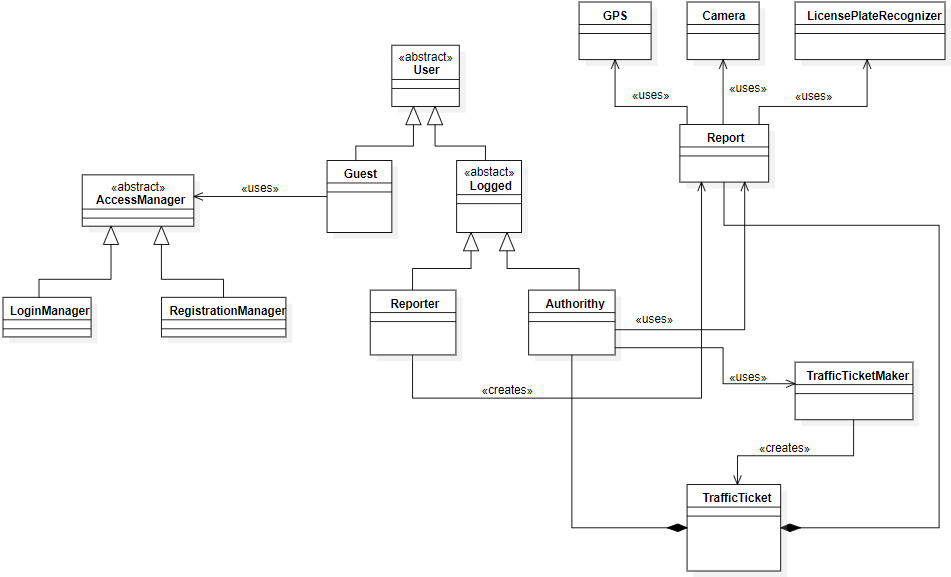
\includegraphics[scale=0.5]{Images/ClassDiag.png}
        \caption{Class Diagram}
    \end{figure}

\newpage

\subsubsection{State Diagrams}
    \begin{figure}[h]
        \centering
        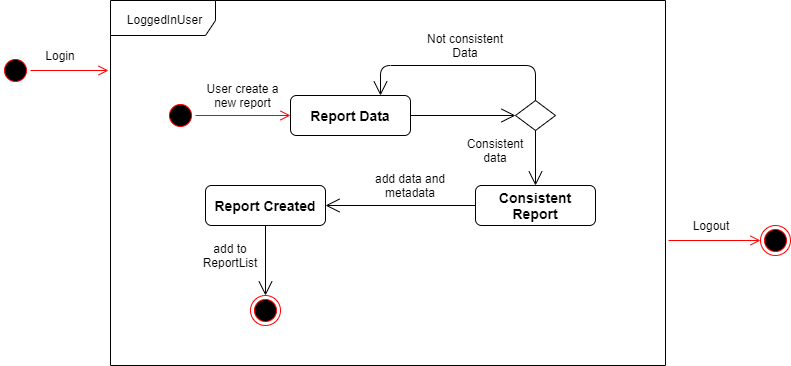
\includegraphics[scale=0.5]{Images/StateDiag_addReport.png}
        \caption{State Diagram of the insertion of a new Report by an User}
    \end{figure}
    
    \vspace{30px}
    
    \begin{figure}[h!]
        \centering
        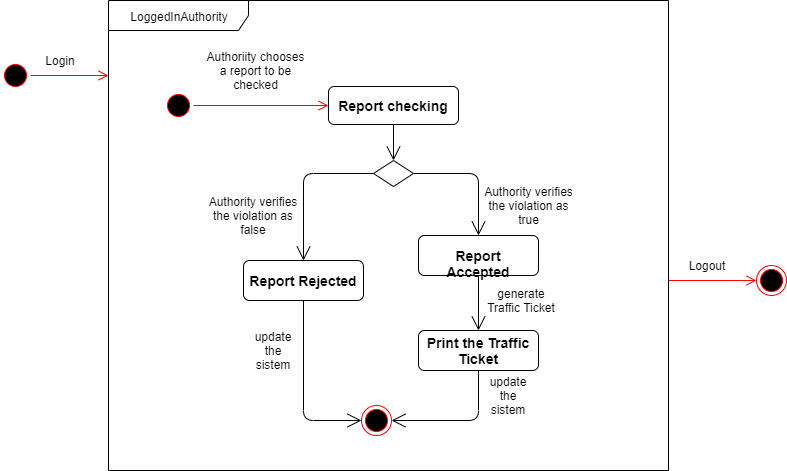
\includegraphics[scale=0.5]{Images/StateDiag_verifyReport.png}
        \caption{State Diagram of the checking of a Report by an Authority}
    \end{figure}


\subsection{Product
functions}

\textbf{SafeStreets}\\
\noindent\textit{SafeStreets} was born with the intention of improving urban traffic mobility, by collecting notifications made by Users about many kinds of traffic violations. Then these information can be consulted by Users themselves, or from Authorities, which can create tickets based on these information.\\ Indeed, \textit{SafeStreets} provides useful suggestions built upon the crossing of Municipality's and \textit{SafeStreets}'s data. \\
Let's see more in the details the functions mentioned above:\\\\

\textbf{Basic User functions} \\
\begin{itemize}
    \item \textbf{Notifying violations}\\\\
    The Users who is witness of a rule violation, and wants to notify it through \textit{SafeStreets}, has to be registered to the application; then he/she can fill up the notification form provided by the application, with a picture of the occurred violation, the kind of violation, the kind of vehicle, the position, (or the address, which can be anyway gathered from GPS), and the license plate of the indeed vehicles.\\
    Not all of these data are mandatory for the User to send, only pictures, GPS position and the kind of violations are: \textit{SafeStreets} uses an algorithm to catch the license plates from the picture, can obtain the address by the GPS position, and uses an algorithm to recognize the vehicles by it self. \textit{SafeStreets} is going to attach these computed metadata to the notification, in case of missing. Time is automatically taken from the notification delivery time.
    
    \item\textbf{Information mined from data}\\\\
    \textit{SafeStreets} provides a friendly interface that allows the User to view Statistics about effectiveness of the application, the most frequent kind of violation and safe and unsafe areas
    
    \end{itemize}  
    
    \textbf{Authority Users functions} \\
    
    \begin{itemize}
   
    
    \item\textbf{SafeStreets suggestion mechanism}\\\\
    The local Municipality provides a way to access their own urban traffic and violations data, \textit{SafeStreets} cross them, to enlarge the amount of information accessible, and exploit them to formulate suggestions for Authorities, in order to increase the functionality of the urban infrastructures, reduce the violations and improve road conditions.\\ Authorities and Municipality can consult these suggestions for various areas, with a function button on the application interface.\\
    Imagine a situation in which \textit{SafeStreets} knows about huge amount of bike lane invasion violations, and municipality knows that in that zone, many people use bikes for moving, then \textit{SafeStreets} can cross those information and provide the suggestion to build a separation line between the car road, and the bike lane, because it should be a good investment, knowing the fact that not only there are lots of violations, but also that those could be very dangerous, given the number of people using bike in that zone. 
    
    
     
    \item\textbf{Searching for violations}\\\\
    In addition to the statistic functions provided for Users, Authorities can also access some more "sensible data", and carry out more precise searches about violations. They can access the list of violations, with relatives license plates and data of involved people.
    Authorities can also use the application to get suggestions about which are the most unsafe urban areas, and how to get them better.
    
    
    \item\textbf{Traffic tickets service}\\\\
    \textit{SafeStreets} allows Authorities the possibility to generate traffic tickets from the violations information sent by Users. An appointee Authority can check a notified violation and all the data attached to it, confirm that it is actually a violation, and then use function provided by \textit{SafeStreets} to generate a ticket. \\
    In order to make this right, \textit{SafeStreets} has to ensure that the chain of custody of the data, from the User to the Authority, is completely reliable. To do this, security algorithms perform a validity check on the sent pictures, to be sure that the picture has not been modified. In case it is, discard the notification. Discarded data are used to make statistical analysis.
    Another filtering level is applied by allowing Users to only send pictures taken while filling up the notification form, and not to upload previously taken ones. In this way, it's harder for a User to modify a picture before sending it. 
\end{itemize}

\newpage
\subsection{User
characteristics}
SafeStreets is an application suitable for every person that possesses a mobile phone.
\subsubsection{Actors}
\begin{itemize}
    \item \textbf{Guest}: a person who downloaded the application and still has to register, he cannot use any functionality of the application.
    \item \textbf{User}: once a guest has registered through the initial form of the application, he gets an account with a \textit{username} and a \textit{password}. Moreover, the User has accepted to give his location and access to the camera of the mobile phone.
    \item \textbf{Authority}: a municipality representative that is able to verify reports and generate traffic tickets from the reported violations. Furthermore, he/she can access to other functionalities that a User cannot even see.
\end{itemize}
\subsection{Assumptions,
dependencies
and
constraints}


\subsubsection{Domain Assumptions}
\begin{itemize}
    \item {[D.1]} Personal data given by Users during the registration process are assumed to be correct.
    \item {[D.2]} Pictures sent by Users are assumed to be in some precise file format.
    \item {[D.3]} The GPS is assumed to be subject to a maximum error of 20 meters.
    \item {[D.4]} Violations for which a ticket is generated, are supposed to be validated by Authorities before.
    \item {[D.5]} Information obtained by Municipality are supposed to be correct.
    \item {[D.6]} Is assumed that there's no bounds which suggestions provided by the S2B have to respect.
    \item {[D.7]} Is assumed that the camera used by the User's device is working properly.
    \item {[D.8]} Is assumed that the GPS module used by the User's device is working properly.
     \item {[D.9]} Is assumed that the municipality offers an API to access their urban mobility data.
    
\end{itemize}

\subsubsection{Dependencies}
\begin{itemize}
    \item The S2B will use the GPS service of the Users smartphone.
    \item The S2B will use the camera function of the Users smartphone.
    \item The S2B will use the internet connectivity of the Users smartphone.
    \item The S2B will use some external API to provide  a map view service to the Users.
    \item The S2B will use the information provided by local municipality, to cross data and create suggestions.
    \item The S2B will use the Authority Traffic Tickets System to generate and send tickets to who has committed violations.\\
\end{itemize}


%\subsubsection{Constraints}




